% !TeX spellcheck = en_US
% !TeX root = ../build/road-to-scalability.tex
% !TeX TXS-program:compile = txs:///xelatex/[--shell-escape]



%%%%%%%%%%%%%%%%%%%%%%%%%%%%%%%%%%%%%%%%%%%%%%%%%%%%%%%%%%%%%%%%%%%%%%%%%%
\section{Introduction}

In our current design, the central entity responsible for assembling batches for sequencing is a \textbf{trusted sequencer}, which is built and managed by Polygon (implemented by us). However, it is prudent to consider the possibility that this sequencer may omit our Layer 2 transactions. In light of this concern, we have implemented anti-censorship mechanisms, which will be discussed in more detail later on.

Figure \ref{fig:seq-system} shows how the Sequence System works.

\begin{figure}[H]
\centering
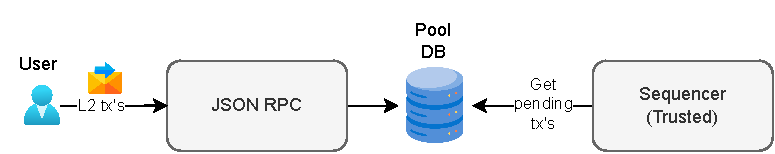
\includegraphics[scale=0.75]{\zkevmdir/figures/architecture/sequencing-batches/sequencer.drawio}
\caption{The user initiates L2 transactions via JSON RPC, directing them to a database known as the \textbf{pool}. Subsequently, the sequencer employs specific criteria to choose a set of pending L2 transactions (those not yet sequenced), aggregates them, and then generates a batch to be sequenced and then proved.}
\label{fig:seq-system}
\end{figure} 




%%%%%%%%%%%%%%%%%%%%%%%%%%%%%%%%%%%%%%%%%%%%%%%%%%%%%%%%%%%%%%%%%%%%%%%%%%%%%
\section {Batch pre-Execution}


The initial step in creating a batch involves verifying that the chosen transactions align with the available execution traces and do not surpass the gas limit. This procedure, known as \textbf{batch pre-execution}, is carried out by the sequencer through an executor as depicted in Figure \ref{fig:batch-pre-ex}. While no proof is generated during this stage, it ensures that the subsequent proof generation process by the prover can be successfully accomplished.

\begin{figure}[H]
\centering
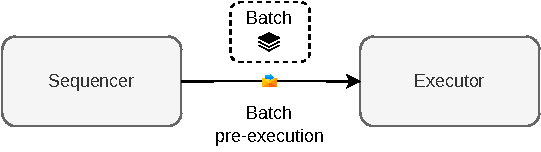
\includegraphics[scale=0.75]{\zkevmdir/figures/architecture/sequencing-batches/batch-preexecution.drawio}
\caption{Batch Pre-Execution is carried by the sequencer through the executor.}
\label{fig:batch-pre-ex}
\end{figure} 


The objective is to expedite the sequencing of batches to enhance the user's perception of speed. Therefore, a \textbf{fast executor} (single-computation executor) is employed, capable of executing within the \texttt{blocktime}. The sequencer communicates with this executor to perform the pre-execution process swiftly. Upon determining the transactions that correctly fill a specific batch through successful batch pre-execution, the sequencer records the batch in the node's StateDB as a \textbf{closed batch}. Closure may occur when the maximum number of execution trace rows is reached, the maximum gas limit is attained, or the allocated time expires.

During the batch pre-execution, for closing the batch the sequencer and the executor also update the Merkle tree of the zkEVM that is stored in the Prover HashDB with L2 state changes, as shown in Figure \ref{fig:close-batch}


\begin{figure}[H]
\centering
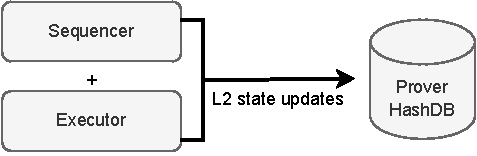
\includegraphics[scale=0.75]{\zkevmdir/figures/architecture/sequencing-batches/batch-closing.drawio}
\caption{The sequencer and the executor store the L2 state updates in the Prover HashDB and the batch is closed.}
\label{fig:close-batch}
\end{figure} 

The throughput of the zkEVM highly depends on the speed at which we are able to close batches which is highly impacted by the batch pre-execution process. So, those involved are the Sequencer, the Executor and the Prover HashDB. In fact, here occur most of the performance problems because interacting to much with the HashDB is inefficient. Currently, efforts are underway to optimize this process by accumulating all changes made to a transaction and updating the HashDB only at the conclusion of the transaction, aiming to mitigate the time spent on frequent updates during transaction processing. 

%añadir lo de grupos?? estos son los l2 blocks pero sse explican luego
%l2 batch is a unit of proving
%l2 block is what a user sees in the system, unit of processing
%each l2 tx is included in its own block, hay tantas tx como blocks, mas adelante agrupamos txs en un block


%%%%%%%%%%%%%%%%%%%%%%%%%%%%%%%%%%%%%%%%%%%%%%%%%%%%%%%%%%%
\section{Send the Sequenced Batch to L1}

The next step is to send a transaction to the Smart Contract to sequence this batch. After the batch is closed, the sequencer stores the data of the batch into the node's StateDB. Then, the \texttt{sequenceSender} looks for closed batches and sends them to L1 Smart contract using the \texttt{EthTxManager}, who makes sure that the transaction is included in a batch. This process is depicted in Figure \ref{fig:seq-tx-L1}

\begin{figure}[H]
\centering
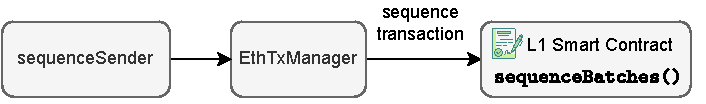
\includegraphics[scale=0.75]{\zkevmdir/figures/architecture/sequencing-batches/sequence-tx-to-L1.drawio}
\caption{The closed batches are sent to L1 by the sequenceSender using the EthTxManager.}
\label{fig:seq-tx-L1}
\end{figure} 

To sequence the batch, the sequencer calls the \texttt{sequenceBatches()} function in the L1 Smart Contract. The name of the function is in plural because we can sequence several batches in a single transaction. This step provides L2 data availability in the L1 execution layer, because we are registering in L1 all the bytes of the L2 transactions.

The calldata for the L1 \texttt{sequenceBatches()} function needs to include the following information: the \textbf{L2 transactions' data}, which is an array containing data for each batch, which encompasses all transactions within the batch along with a timestamp indicating its closure time. Additionally, the \textbf{L2 coinbase address}, representing the Ethereum address for receiving user fees. Lastly, a \textbf{timestamp} indicating when the L2 transactions were sequenced.

The L2 coinbase address serves as a critical destination for rewards earned by the sequencer in the Layer 2 environment. The sequencer undertakes the responsibility of paying for data availability in Layer 1 using L1 Ether. When the sequencer successfully closes a batch and executes transactions, they receive a reward for their services. This reward, denominated in L2 Ether, is routed to the L2 coinbase address.

Crucially, the L2 coinbase address is situated within Layer 2 because users compensate the sequencer with L2 Ether. This L2 Ether, representing the reward, is a reflection of the Ether in L1 that users have previously transferred to L2 through transactions via the Bridge. Importantly, there exists a direct and fixed 1:1 correspondence between L1 ETH and L2 ETH, as we can observe in Figure \ref{fig:ether}.

\begin{figure}[H]
\centering
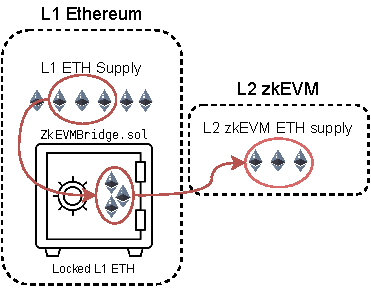
\includegraphics[scale=0.75]{\zkevmdir/figures/architecture/sequencing-batches/l2-ether.drawio}
\caption{Ethter of L1 and L2 is equivalent.}
\label{fig:ether}
\end{figure} 




%%%%%%%%%%%%%%%%%%%%%%%%%%%%%%%%%%%%%%%%%%%%%%%%%%%%%%%%%%%%%
\section{Accumulated Input Hash Pointers}

Examining the sequencing process in more detail, when the Smart Contract receives a transaction for sequencing, it initiates the creation of cryptographic pointers for each batch. These pointers play a crucial role in uniquely identifying a batch, specifying its position, and encapsulating its data. Subsequently, provers utilize these pointers as references during the proofing process, allowing them to precisely identify and retrieve the batch being proved along with its associated data. This systematic use of cryptographic pointers ensures a robust and unambiguous linkage between the sequencing transaction and the corresponding batch data for subsequent verification.

\begin{figure}[H]
\centering
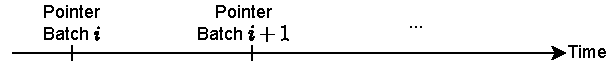
\includegraphics[scale=0.9]{\zkevmdir/figures/architecture/sequencing-batches/pointer-line-time.pdf}
\caption{Generation of Pointers in a line time.}
\label{fig:pointer-line-time}
\end{figure} 

These pointers are constructed using a hash that accumulates data, incorporating information from all preceding blocks. The procedural steps for this process are illustrated in Figure \ref{fig:accinputhash-pointers}:

\begin{figure}[H]
\centering
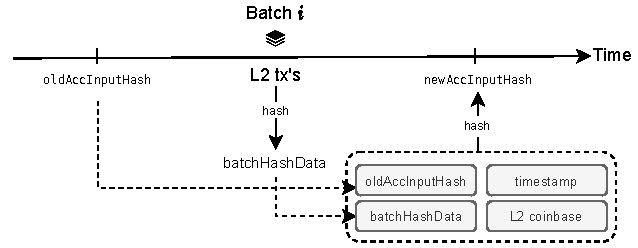
\includegraphics[scale=0.9]{\zkevmdir/figures/architecture/sequencing-batches/accHash-line-time}
\caption{The new cryptographic pointer is created with the hashed data of the previous one, among other.}
\label{fig:accinputhash-pointers}
\end{figure} 

Indeed, as depicted in Figure \ref{fig:pointer-line-time}, pointers are generated by executing a KECCAK hash on several components, including the previous pointer, the transactions encompassed within the L2 batch, the batch timestamp and the L2 coinbase. Due to the interconnected nature of their creation, with each pointer encapsulating the previous one in the input of the hash, they are aptly referred to as \textit{accumulated input hash} or \texttt{accInputHash}. This linked construction is imperative to guarantee that the data of batches is proven in the correct sequential order.


Upon the completion of the sequencing process, the batch enters a state of being \textit{virtualized}, residing within the previously discussed Virtual State. 







